% !TeX root = ../../thesis.tex
\chapter{Fluid flow and convection}\label{ch:fluid}

\section{Introduction}

\begin{figure}[h]
\centering
\medskip
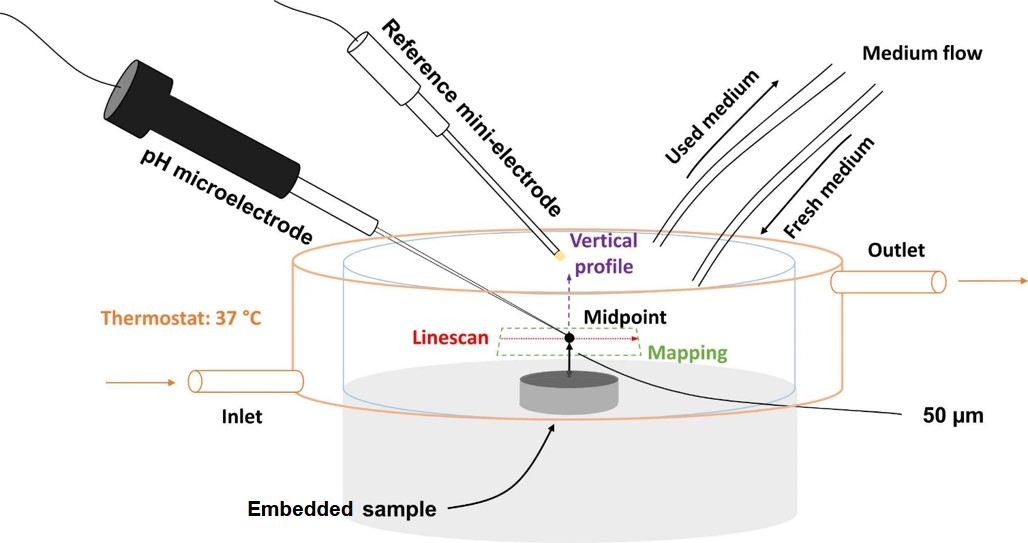
\includegraphics[width=\textwidth]{setup.jpg}
\caption[Fluid flow model construction for comparison with experimental setup]{Fluid flow model construction for comparison with experimental setup} \label{fig:fluid_setup}
\end{figure}

\begin{figure}[h]
\centering
\medskip
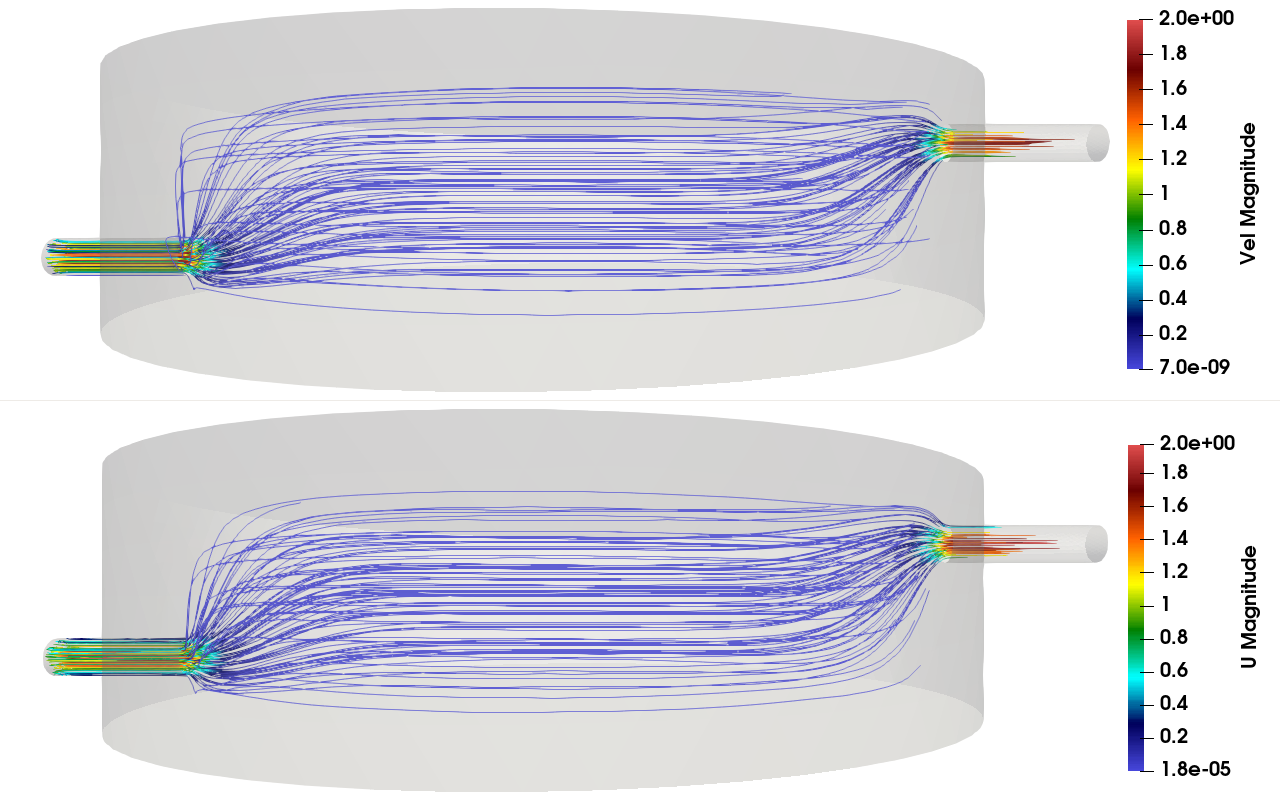
\includegraphics[width=\textwidth]{streamlines_side.png}
\caption[Comparing streamline results of developed CFD code and OpenFOAM - side view]{Comparing streamline results of developed CFD code and OpenFOAM - side view} \label{fig:fluid_streamlines_side}
\end{figure}


\begin{figure}[h]
\centering
\medskip
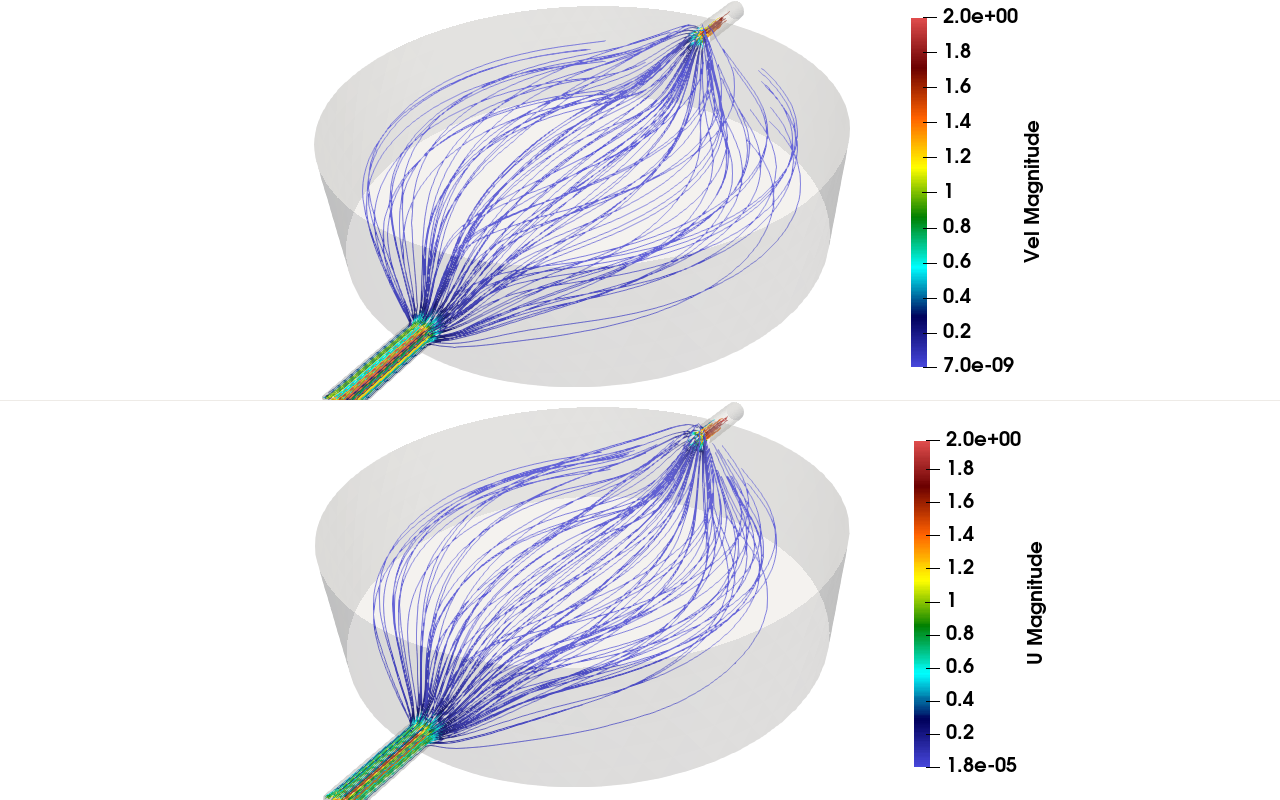
\includegraphics[width=\textwidth]{streamlines_top.png}
\caption[Comparing streamline results of developed CFD code and OpenFOAM - top view]{Comparing streamline results of developed CFD code and OpenFOAM - top view} \label{fig:fluid_streamlines_top}
\end{figure}


\begin{figure}[h]
\centering
\medskip
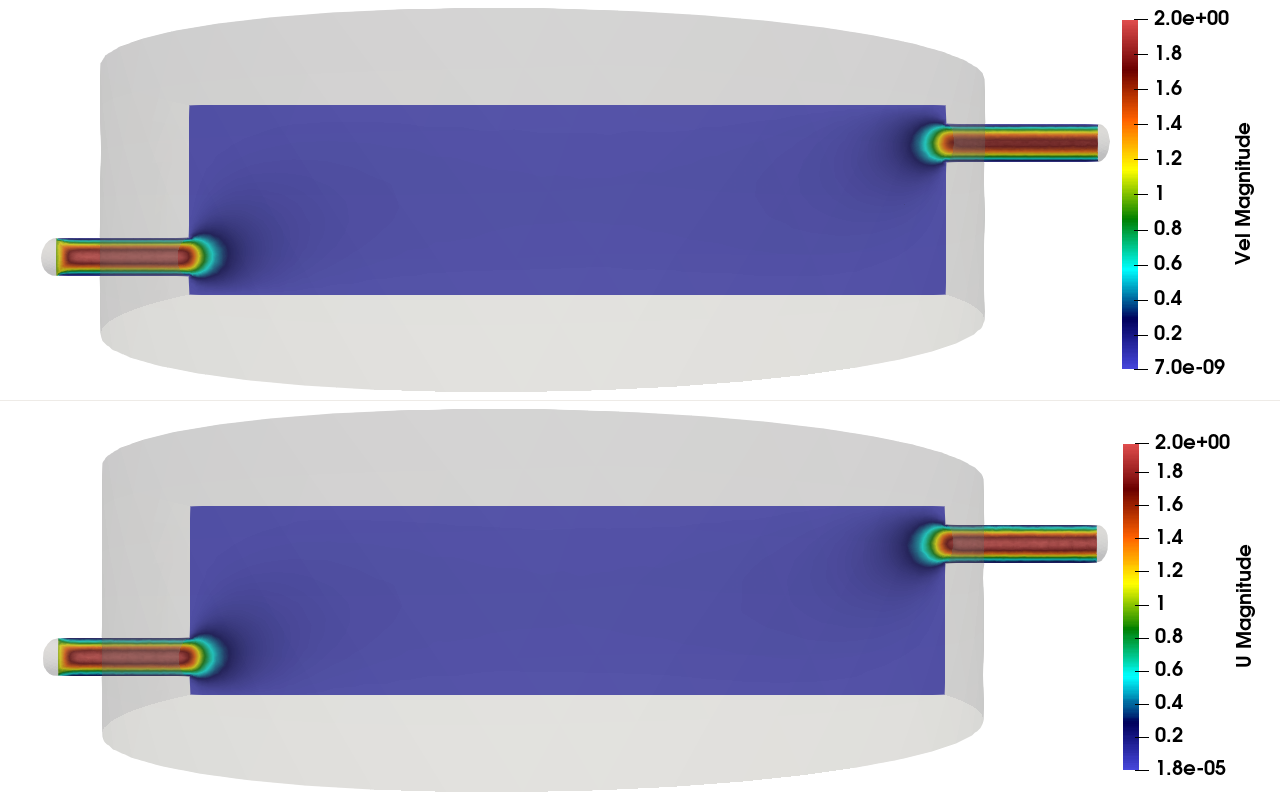
\includegraphics[width=\textwidth]{flow_chamber.png}
\caption[Comparing flow field results of developed CFD code and OpenFOAM]{Comparing streamline results of developed CFD code and OpenFOAM} \label{fig:fluid_flow_chamber}
\end{figure}


\begin{figure}[h]
\centering
\medskip
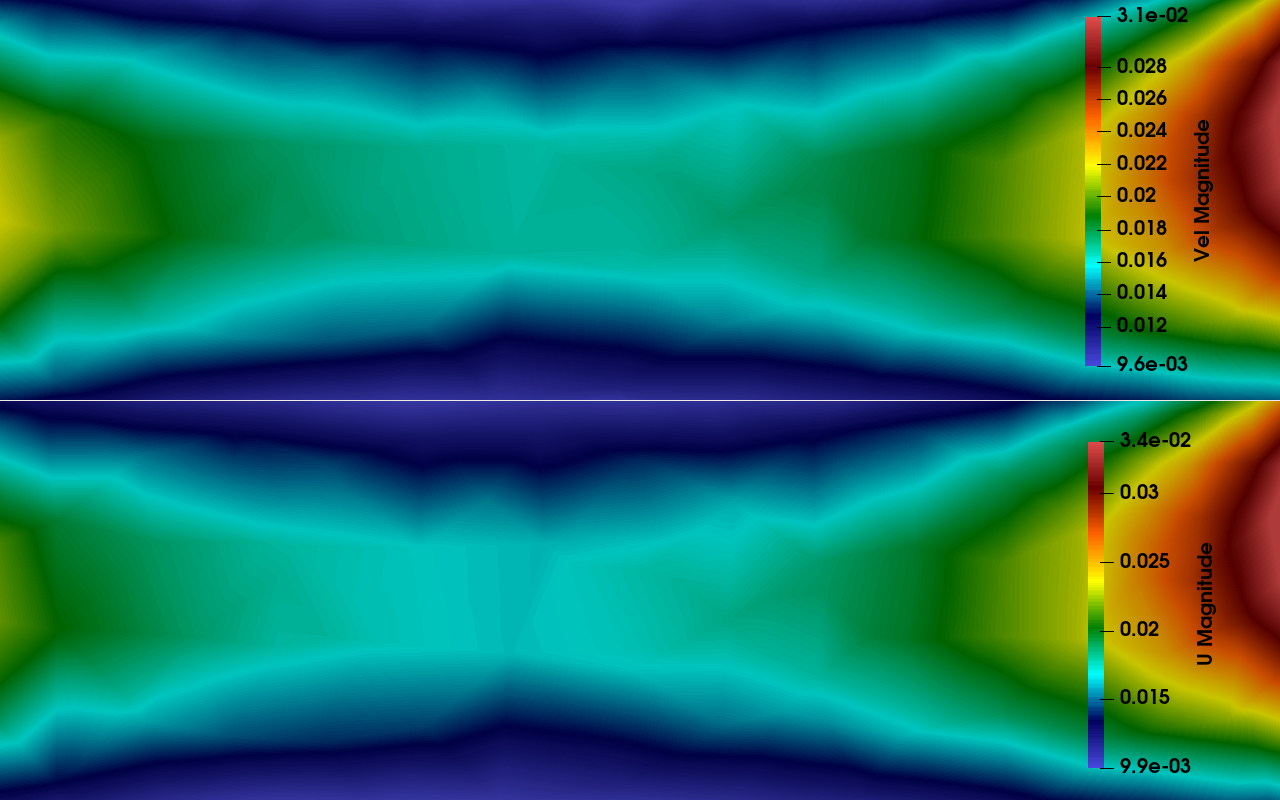
\includegraphics[width=\textwidth]{flow_chamber_zoom.png}
\caption[Comparing flow field results of developed CFD code and OpenFOAM - zoomed view]{Comparing streamline results of developed CFD code and OpenFOAM - zoomed view} \label{fig:fluid_flow_chamber_zoom}
\end{figure}

\begin{figure}[h]
\centering
\medskip
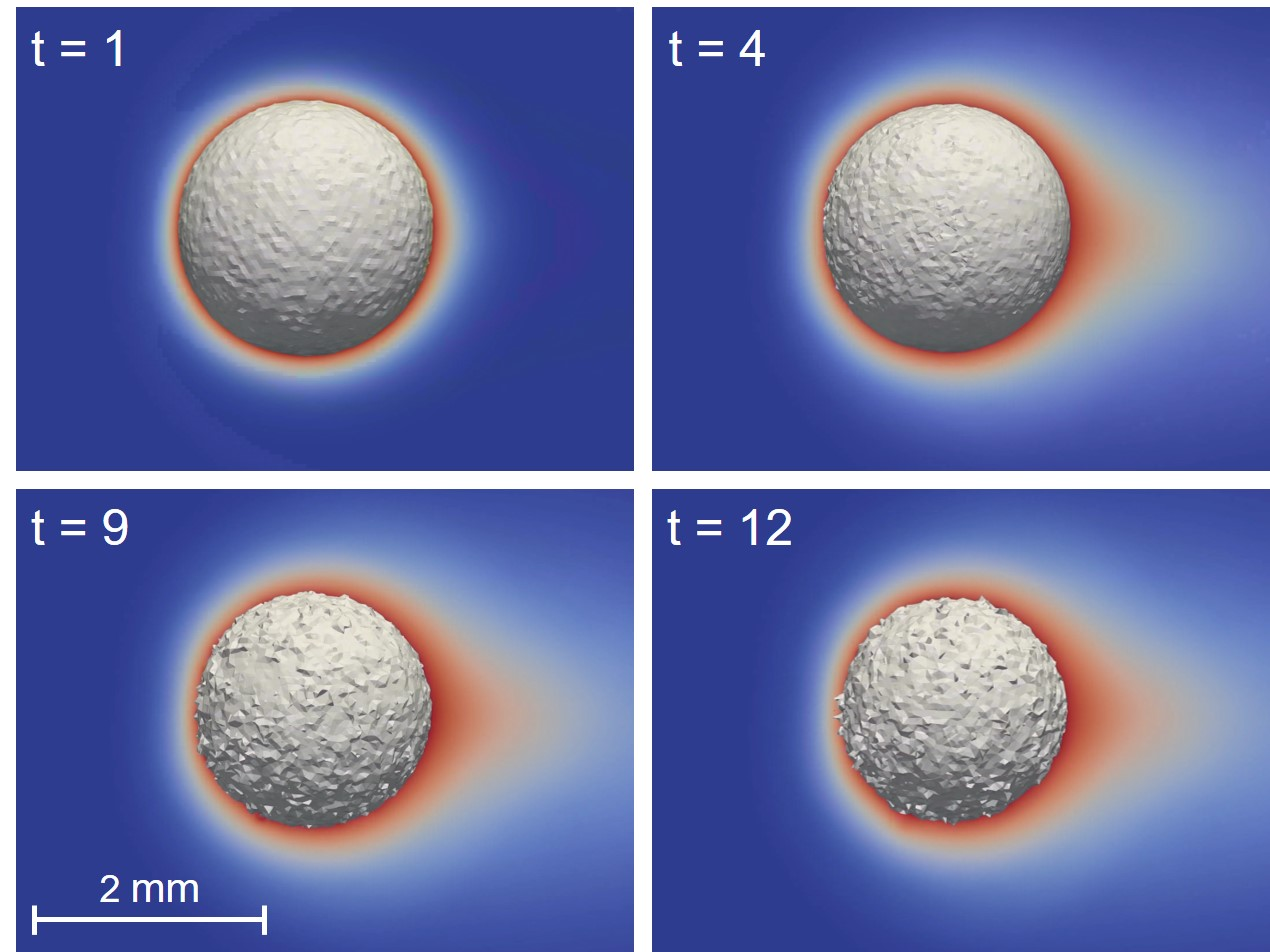
\includegraphics[width=\textwidth]{flow_degrading.jpg}
\caption[Biodegradation simulation results in the presence of fluid flow]{Biodegradation simulation results in the presence of fluid flow} \label{fig:fluid_flow_degrading}
\end{figure}


\begin{figure}[h]
\centering
\medskip
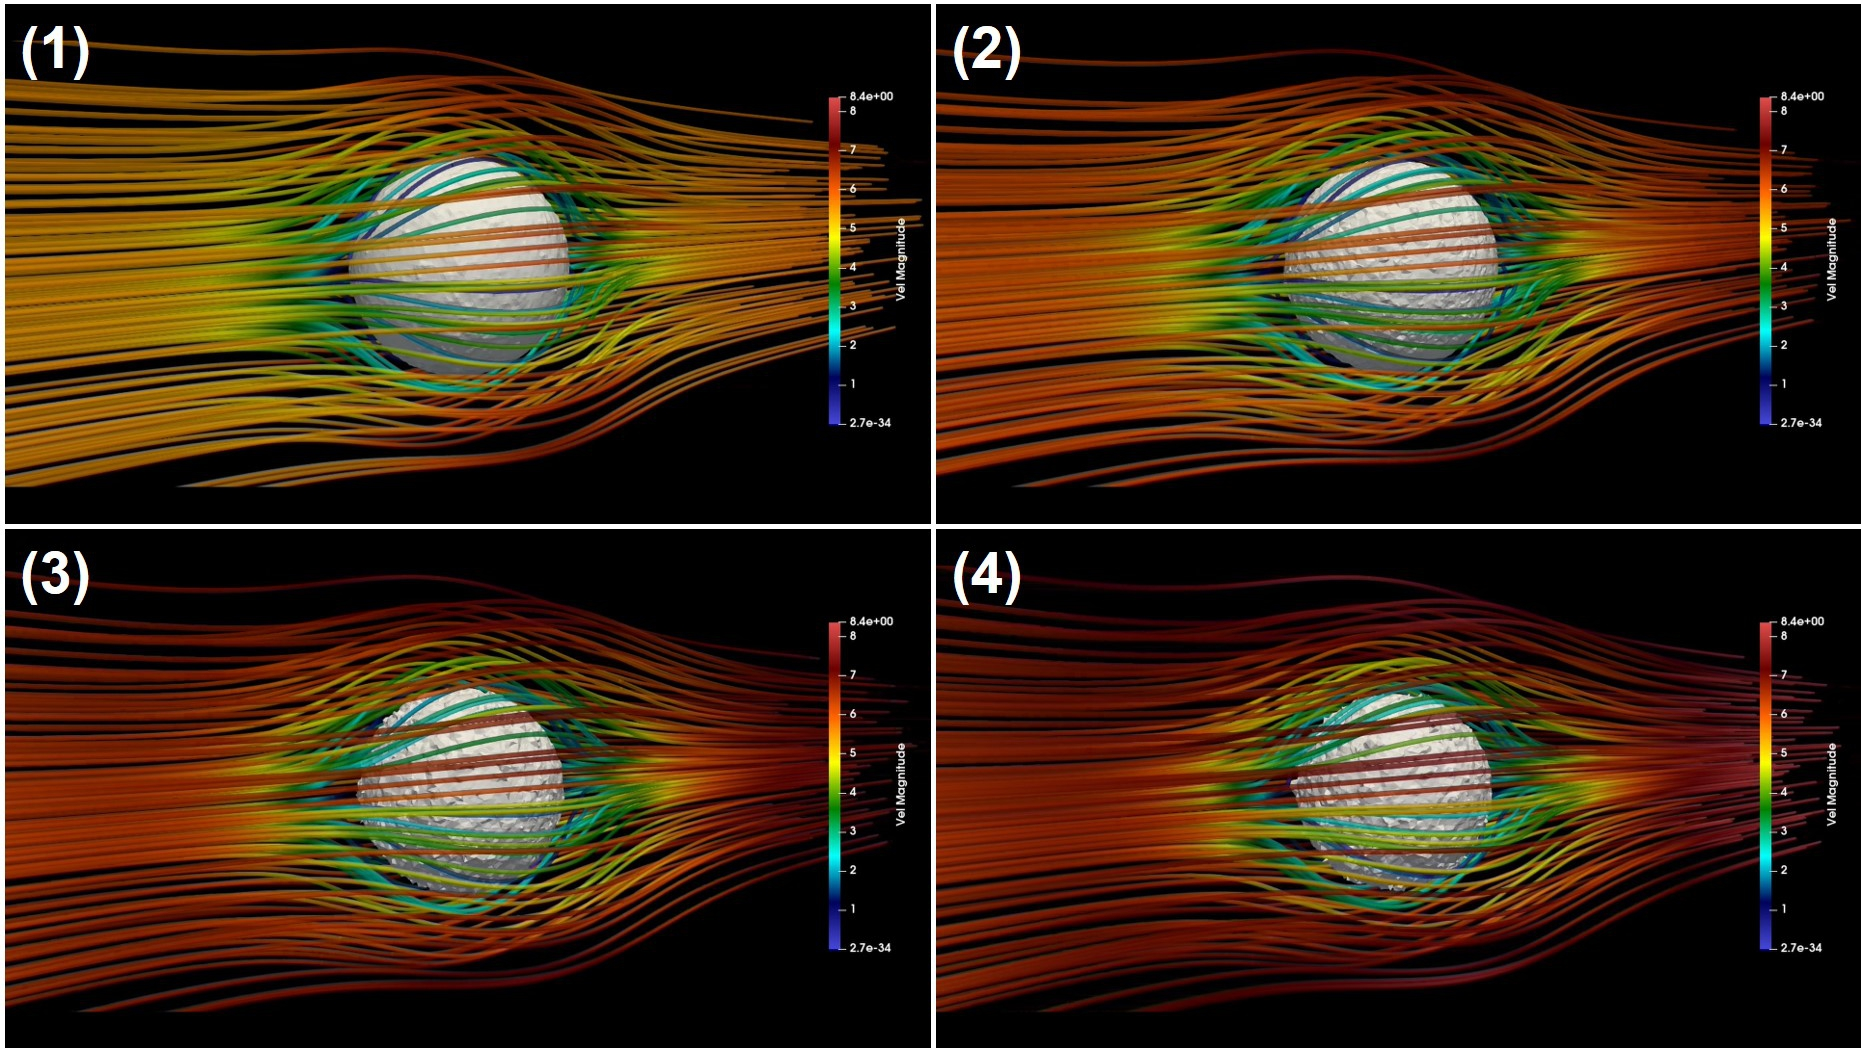
\includegraphics[width=\textwidth]{flow_degrading_streamline.jpg}
\caption[Fluid flow streamlines in the presence of a degrading object]{Fluid flow streamlines in the presence of a degrading object} \label{fig:fluid_flow_degrading_streamline}
\end{figure}
















%%%%%%%%%%%%%%%%%%%%%%%%%%%%%%%%%%%%%%%%%%%%%%%%%%
% Keep the following \cleardoublepage at the end of this file, 
% otherwise \includeonly includes empty pages.
\cleardoublepage

